\documentclass[12pt,b5paper]{ltjsarticle}

\usepackage[margin=15truemm]{geometry}
\pagestyle{empty}

\usepackage{amssymb}
\usepackage{amsmath}	% required for `\align' (yatex added)

\usepackage{graphicx}	% required for `\includegraphics' (yatex added)
\usepackage{wrapfig}	% required for `\wrapfigure' (yatex added)
\begin{document}

二次関数$y=2x^2$のグラフと直線$l$の交点$A(2,8),B(-1,?)$について
\begin{enumerate}
 \item 点$B$

       $y=2x^2$に$x=-1$を代入する。

       \underline{$B(-1,2)$}
 \item 直線$l$の式

       直線$l$の式を$y=ax+b$と表す。
       $l$は$A,B$を通るのでこの2つの座標を
       $y=ax+b$に代入する。
       \begin{align}
        (x,y)=(2,8)を代入 \qquad 8=& a\times 2 +b\\
        (x,y)=(-1,2)を代入 \qquad 2=& a \times (-1) +b
       \end{align}
       得られた式を整理すると
       \begin{equation}
        \begin{cases}
         2a+b=8\\
         -a+b=2
        \end{cases}
       \end{equation}
       得られた式の連立方程式を解くと
       \begin{equation}
        a=2, \quad b=4
       \end{equation}
       が分かる。
       これを直線$l$の式に代入すると次の式が求まる。
       \underline{$y=2x+4$}
       
 \item $\triangle OAB$の面積


       図の青い四角の面積を求めそこから
       $\triangle OAB$の外側の面積を引くと求められる。

       四角形の面積は$3\times8=24$

       取り除く三角形は3つあり、
       それぞれの面積は
       $1\times2\div2=1$、
       $2\times8\div2=8$、
       $3\times6\div2=9$
       である。

       $\triangle OAB$の面積は
       $24-1-8-9=\underline{6}$である。

\end{enumerate}

%       \begin{wrapfigure}{R}{30mm}
        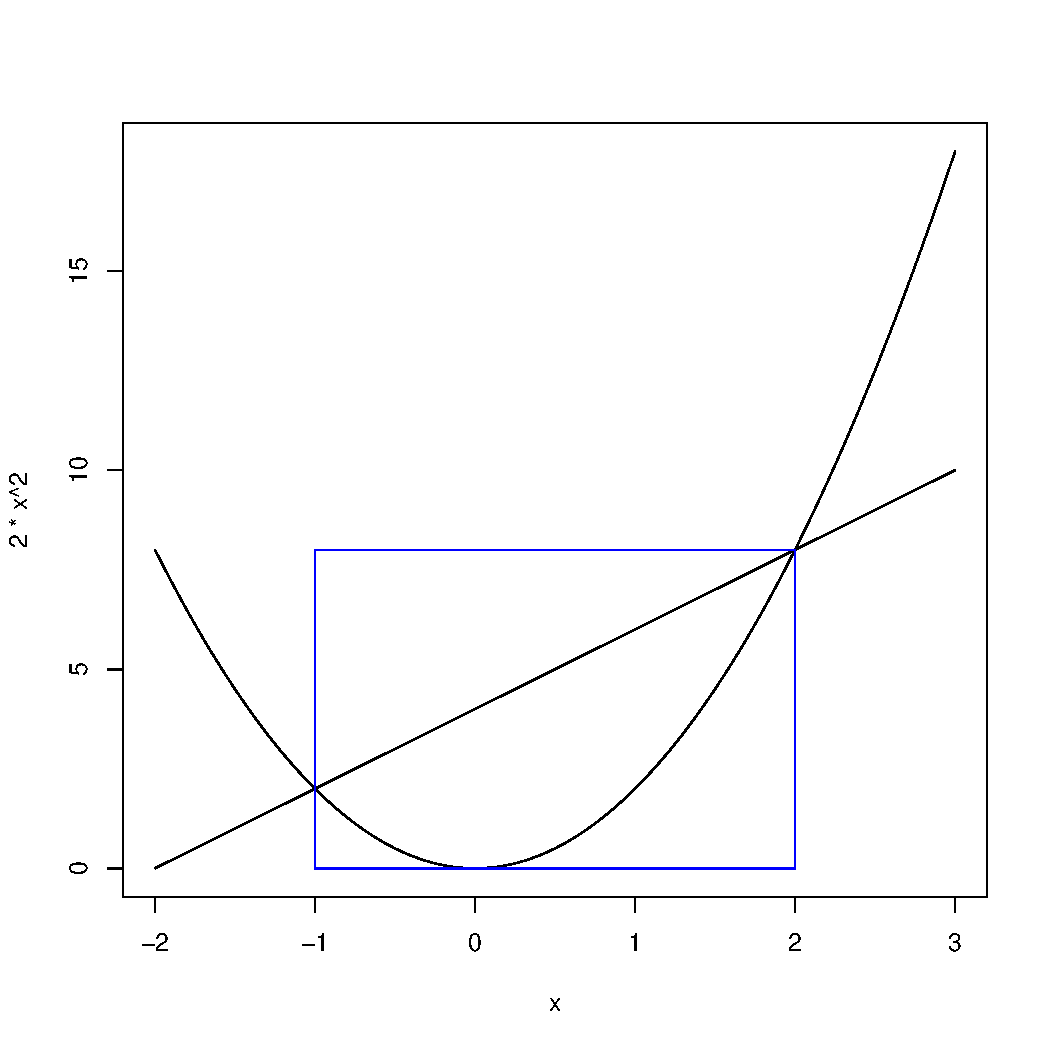
\includegraphics[scale=0.3]{graph.pdf}
%       \end{wrapfigure}





\end{document}
